\textbf{Ejemplo 5}\\
Hallar el monto, el valor futuro y el valor presente de 20 pagos de 200.000 COP cada uno, suponga una tasa del 24\% nominal anual año vencido.\\ \\
%\newpage %USAR SOLO SI EL SOLUCIÓN QUEDA SOLO Y ES NECESARIO BAJARLO A LA SIGUIENTE PAGINA
\textbf{Solución.}
%La tabla ira centrada
\begin{center}
 \renewcommand{\arraystretch}{1.5}% Margenes de las celdas
 %Creación de la cuadricula de 3 columnas
 \begin{longtable}[H]{|p{0.333\linewidth}|p{0.3333\linewidth}|p{0.3333\linewidth}|}
  \hline
  \multicolumn{3}{|c|}{\cellcolor[HTML]{FFB183}\textbf{1. Declaración de variables}}                   \\ \hline
  $R= 200.000 COP$         & $i=24\% \hspace{1mm} pav$ & $VP = ? COP$                                  \\
  $n=20 \hspace{1mm} pav$ &                            & $VF= ? COP$                                   \\ \hline
  \multicolumn{3}{|c|}{\cellcolor[HTML]{FFB183}\textbf{2. Tabla de flujo de caja}}                     \\ \hline
  \multicolumn{3}{|p{\columnwidth}|}{
  \begin{center}
   \begin{tabular}{ |p{3.5cm}| p{3cm}|}
    \hline

    \textbf{Periodo (psv) } & \textbf{Flujo} \\ \hline
    0                       & -              \\\hline
    1                       &  200.000 COP     \\ \hline
    2                       &  200.000 COP     \\ \hline
    3                       &  200.000 COP     \\ \hline
    4                       &  200.000 COP     \\ \hline
    5                       &  200.000 COP     \\ \hline
    6                       &  200.000 COP     \\ \hline
    7                       &  200.000 COP     \\ \hline
    8                       &  200.000 COP     \\ \hline
    9                       &  200.000 COP     \\ \hline
    10                      &  200.000 COP     \\ \hline
    11                      &  200.000 COP     \\ \hline
    12                      &  200.000 COP     \\ \hline
    13                      &  200.000 COP     \\ \hline
    14                      &  200.000 COP     \\ \hline
    15                      &  200.000 COP     \\ \hline
    16                      &  200.000 COP     \\ \hline
    17                      &  200.000 COP     \\ \hline
    18                      &  200.000 COP     \\ \hline
    19                      &  200.000 COP     \\ \hline
    20                      &  200.000 COP     \\ \hline
   \end{tabular}

  \end{center}
  }                                                                                                   \\ \hline
  \multicolumn{3}{|c|}{\cellcolor[HTML]{FFB183}\textbf{3. Fórmulas utilizadas}}                       \\ \hline
  \multicolumn{3}{|p{\columnwidth}|}{Mediante el uso de Excel:
  \begin{itemize}
   \item VA (Valor actual): Devuelve el valor presente para una inversión
   \item VF (Valor Futuro): Devuelve el valor futuro de una inversión basado en pagos
         periódicos y constantes, y una tasa de interés constante
  \end{itemize}
  }                                                                                                   \\ \hline
  \multicolumn{3}{|c|}{\cellcolor[HTML]{FFB183}\textbf{4. Desarrollo en Excel}}                       \\ \hline
  \multicolumn{3}{|l|}{Se aplicarán las funciones VA y VF de la siguiente forma:}                     \\
  \multicolumn{3}{|c|}{ 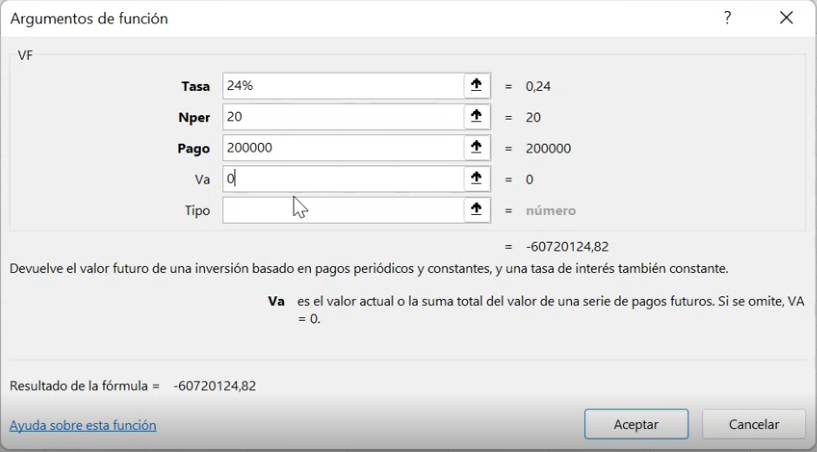
\includegraphics[trim=-5 -5 -5 -5 ,width=1\columnwidth]{5/Ejem5.1.PNG}}        \\
  \multicolumn{3}{|l|}{=VF(0,24;20;-200000;0) con referencia en la hoja de Excel usada para el ejercicio.}    \\
  \multicolumn{3}{|c|}{ 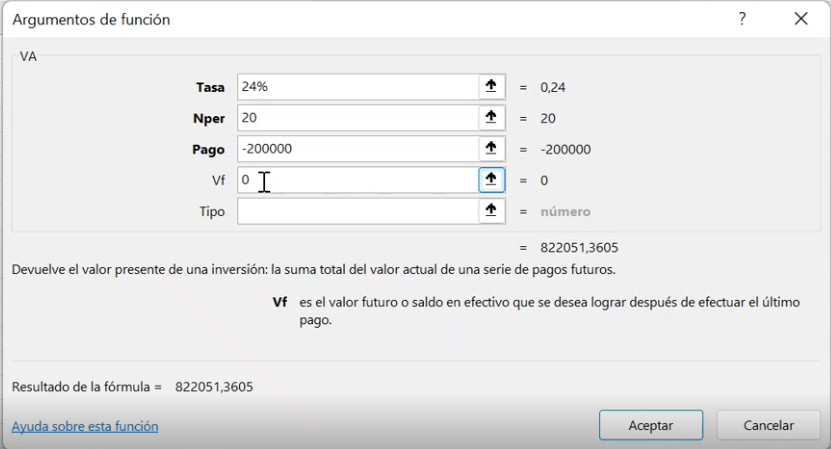
\includegraphics[trim=-5 -5 -5 -5 ,width=1\columnwidth]{5/Ejem5.2.PNG}}        \\
  \multicolumn{3}{|l|}{=VA(0,24;20;-200000;0) con referencia en la hoja de Excel usada para el ejercicio.} \\ \hline
  \multicolumn{3}{|c|}{\cellcolor[HTML]{FFB183}\textbf{5. Respuesta}}                                 \\ \hline
  \multicolumn{3}{|p{\columnwidth}|}{
  El valor presente (VP) o valor actual (VA) es 822.051 COP y el valor futuro (VF) es 60.720.114 COP 
  }                                                                                                   \\ \hline
  \multicolumn{3}{|c|}{\cellcolor[HTML]{FFB183}\textbf{6. Gráfica}}                                   \\ \hline
  \multicolumn{3}{|c|}{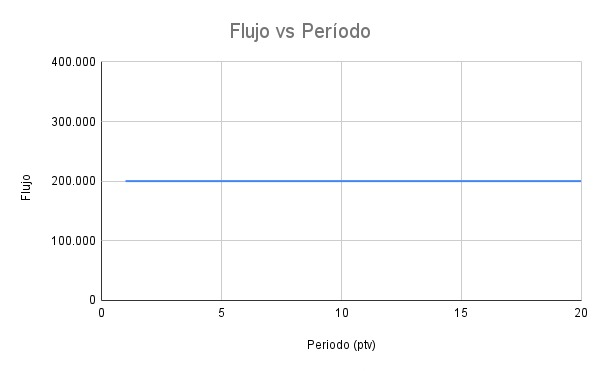
\includegraphics[trim=-5 -5 -5 -5 ,width=0.7\columnwidth]{4/flujovsperiodo.png}}      \\ \hline
 \end{longtable}
 %\newline \newline %USARLO SI CREES QUE ES NECESARIO
\end{center}
